% Options for packages loaded elsewhere
\PassOptionsToPackage{unicode}{hyperref}
\PassOptionsToPackage{hyphens}{url}
%
\documentclass[
  ignorenonframetext,
]{beamer}
\usepackage{pgfpages}
\setbeamertemplate{caption}[numbered]
\setbeamertemplate{caption label separator}{: }
\setbeamercolor{caption name}{fg=normal text.fg}
\beamertemplatenavigationsymbolsempty
% Prevent slide breaks in the middle of a paragraph
\widowpenalties 1 10000
\raggedbottom
\setbeamertemplate{part page}{
  \centering
  \begin{beamercolorbox}[sep=16pt,center]{part title}
    \usebeamerfont{part title}\insertpart\par
  \end{beamercolorbox}
}
\setbeamertemplate{section page}{
  \centering
  \begin{beamercolorbox}[sep=12pt,center]{part title}
    \usebeamerfont{section title}\insertsection\par
  \end{beamercolorbox}
}
\setbeamertemplate{subsection page}{
  \centering
  \begin{beamercolorbox}[sep=8pt,center]{part title}
    \usebeamerfont{subsection title}\insertsubsection\par
  \end{beamercolorbox}
}
\AtBeginPart{
  \frame{\partpage}
}
\AtBeginSection{
  \ifbibliography
  \else
    \frame{\sectionpage}
  \fi
}
\AtBeginSubsection{
  \frame{\subsectionpage}
}
\usepackage{amsmath,amssymb}
\usepackage{lmodern}
\usepackage{ifxetex,ifluatex}
\ifnum 0\ifxetex 1\fi\ifluatex 1\fi=0 % if pdftex
  \usepackage[T1]{fontenc}
  \usepackage[utf8]{inputenc}
  \usepackage{textcomp} % provide euro and other symbols
\else % if luatex or xetex
  \usepackage{unicode-math}
  \defaultfontfeatures{Scale=MatchLowercase}
  \defaultfontfeatures[\rmfamily]{Ligatures=TeX,Scale=1}
  \setmainfont[BoldFont = SF Pro Rounded Semibold]{SF Pro Rounded}
  \setmathfont[]{STIX Two Math}
\fi
\usefonttheme{serif} % use mainfont rather than sansfont for slide text
% Use upquote if available, for straight quotes in verbatim environments
\IfFileExists{upquote.sty}{\usepackage{upquote}}{}
\IfFileExists{microtype.sty}{% use microtype if available
  \usepackage[]{microtype}
  \UseMicrotypeSet[protrusion]{basicmath} % disable protrusion for tt fonts
}{}
\makeatletter
\@ifundefined{KOMAClassName}{% if non-KOMA class
  \IfFileExists{parskip.sty}{%
    \usepackage{parskip}
  }{% else
    \setlength{\parindent}{0pt}
    \setlength{\parskip}{6pt plus 2pt minus 1pt}}
}{% if KOMA class
  \KOMAoptions{parskip=half}}
\makeatother
\usepackage{xcolor}
\IfFileExists{xurl.sty}{\usepackage{xurl}}{} % add URL line breaks if available
\IfFileExists{bookmark.sty}{\usepackage{bookmark}}{\usepackage{hyperref}}
\hypersetup{
  pdftitle={444 Lecture 4.1 - Information Sets},
  pdfauthor={Brian Weatherson},
  hidelinks,
  pdfcreator={LaTeX via pandoc}}
\urlstyle{same} % disable monospaced font for URLs
\newif\ifbibliography
\usepackage{graphicx}
\makeatletter
\def\maxwidth{\ifdim\Gin@nat@width>\linewidth\linewidth\else\Gin@nat@width\fi}
\def\maxheight{\ifdim\Gin@nat@height>\textheight\textheight\else\Gin@nat@height\fi}
\makeatother
% Scale images if necessary, so that they will not overflow the page
% margins by default, and it is still possible to overwrite the defaults
% using explicit options in \includegraphics[width, height, ...]{}
\setkeys{Gin}{width=\maxwidth,height=\maxheight,keepaspectratio}
% Set default figure placement to htbp
\makeatletter
\def\fps@figure{htbp}
\makeatother
\setlength{\emergencystretch}{3em} % prevent overfull lines
\providecommand{\tightlist}{%
  \setlength{\itemsep}{0pt}\setlength{\parskip}{0pt}}
\setcounter{secnumdepth}{-\maxdimen} % remove section numbering
\let\Tiny=\tiny

 \setbeamertemplate{navigation symbols}{} 

% \usetheme{Madrid}
 \usetheme[numbering=none, progressbar=foot]{metropolis}
 \usecolortheme{wolverine}
 \usepackage{color}
 \usepackage{MnSymbol}
% \usepackage{movie15}

\usepackage{amssymb}% http://ctan.org/pkg/amssymb
\usepackage{pifont}% http://ctan.org/pkg/pifont
\newcommand{\cmark}{\ding{51}}%
\newcommand{\xmark}{\ding{55}}%

\DeclareSymbolFont{symbolsC}{U}{txsyc}{m}{n}
\DeclareMathSymbol{\boxright}{\mathrel}{symbolsC}{128}
\DeclareMathAlphabet{\mathpzc}{OT1}{pzc}{m}{it}

\setlength{\parskip}{1ex plus 0.5ex minus 0.2ex}

\AtBeginSection[]
{
\begin{frame}
	\Huge{\color{darkblue} \insertsection}
\end{frame}
}

\renewenvironment*{quote}	
	{\list{}{\rightmargin   \leftmargin} \item } 	
	{\endlist }

\definecolor{darkgreen}{rgb}{0,0.7,0}
\definecolor{darkblue}{rgb}{0,0,0.8}

\usepackage[italic]{mathastext}
\usepackage{nicefrac}

\setbeamertemplate{caption}{\raggedright\insertcaption}

%\def\toprule{}
%\def\bottomrule{}
%\def\midrule{}
\usepackage{etoolbox}
\AfterEndEnvironment{description}{\vspace{9pt}}
\AfterEndEnvironment{oltableau}{\vspace{9pt}}
\BeforeBeginEnvironment{oltableau}{\vspace{9pt}}
\AfterEndEnvironment{center}{\vspace{9pt}}
\BeforeBeginEnvironment{tabular}{\vspace{9pt}}
\AfterEndEnvironment{longtable}{\vspace{-6pt}}
\usepackage{booktabs}
\usepackage{longtable}
\usepackage{array}
\usepackage{multirow}
\usepackage{wrapfig}
\usepackage{float}
\usepackage{colortbl}
\usepackage{pdflscape}
\usepackage{tabu}
\usepackage{threeparttable} 
\usepackage{threeparttablex} 
\usepackage[normalem]{ulem} 
\usepackage{makecell}
\usepackage{xcolor}
\usepackage{ulem}

\setlength\heavyrulewidth{0ex}
\setlength\lightrulewidth{0.08ex}

\aboverulesep=0ex
\belowrulesep=0ex
\renewcommand{\arraystretch}{1.2}
\ifluatex
  \usepackage{selnolig}  % disable illegal ligatures
\fi

\title{444 Lecture 4.1 - Information Sets}
\author{Brian Weatherson}
\date{}

\begin{document}
\frame{\titlepage}

\begin{frame}{Plan}
\protect\hypertarget{plan}{}
To discuss how we introduce uncertainty into the theory of games.
\end{frame}

\begin{frame}{Reading}
\protect\hypertarget{reading}{}
Bonanno, section 4.1; the slide numbers and the section numbers have
joined for now.
\end{frame}

\begin{frame}{Basic Idea}
\protect\hypertarget{basic-idea}{}
\begin{itemize}
\tightlist
\item
  Sometimes when a player has to make a choice, they know they are at
  one of a set of nodes in the tree, but they don't know which one.
\item
  We will illustrate this by drawing a circle around the nodes.
\item
  The circle means that the player making a choice knows that they are
  in that circle somewhere, but the rules of the game don't guarantee
  that they know which point they are in.
\end{itemize}
\end{frame}

\begin{frame}{Cheating Game}
\protect\hypertarget{cheating-game}{}
\begin{itemize}
\tightlist
\item
  Professor decides to either give every student the same exam, or give
  different exams to different students.
\item
  Student doesn't know what professor did, and has to decide whether to
  copy off (known to be good at the course) neighbour.
\end{itemize}
\end{frame}

\begin{frame}
\begin{figure}
\centering
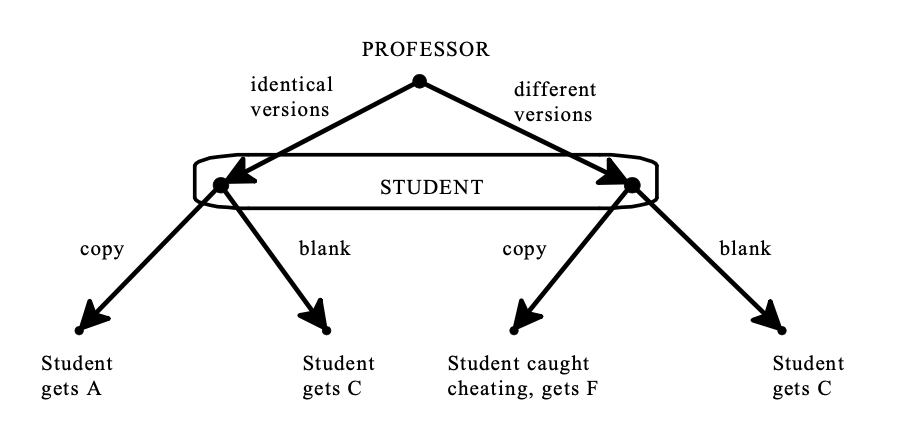
\includegraphics{images/04_01.png}
\caption{Payoff tree for cheating game}
\end{figure}
\end{frame}

\begin{frame}{How To Read Tree}
\protect\hypertarget{how-to-read-tree}{}
\begin{itemize}
\tightlist
\item
  Professor makes a choice.
\item
  Then student makes a choice.
\item
  When student chooses, there is a fact about where in the tree we are.
\item
  But student isn't told that fact - they are just told that we are at
  one of the nodes in the circled set.
\end{itemize}
\end{frame}

\begin{frame}{Circles Everywhere}
\protect\hypertarget{circles-everywhere}{}
\begin{itemize}
\tightlist
\item
  We don't normally draw them, but you should imagine these circles
  everywhere on the tree.
\item
  If a node doesn't have a circle around it, that means that its circle
  just contains itself.
\end{itemize}
\end{frame}

\begin{frame}{Information Set}
\protect\hypertarget{information-set}{}
\begin{itemize}
\tightlist
\item
  We will call the circle associate with each point its
  \textbf{information set}.
\item
  Each node is in precisely one information set.
\item
  That set may be a singleton; it might just be that node.
\item
  But that's not the general case.
\end{itemize}
\end{frame}

\begin{frame}{Constraints on Information Sets - Outputs}
\protect\hypertarget{constraints-on-information-sets---outputs}{}
Every node in an information set must have the same outputs.

\begin{itemize}
\tightlist
\item
  You can't have an information set where the Player has three options
  from one node, but only two from another.
\item
  The player knows how many options they have.
\item
  So if the options were different, they could figure out which node
  they were at.
\end{itemize}
\end{frame}

\begin{frame}{Constraints on Information Sets - Inputs}
\protect\hypertarget{constraints-on-information-sets---inputs}{}
Every node in an information set has the same history of moves by the
player whose turn it is.

\begin{itemize}
\tightlist
\item
  We assume everyone knows what moves they have made.
\item
  It is an interesting fact that some real life board games rely on the
  falsity of this assumption.
\item
  But as on previous slide, if the nodes have a different history for
  this player, that means the player knows which node they are at.
\end{itemize}
\end{frame}

\begin{frame}{For Next Time}
\protect\hypertarget{for-next-time}{}
\begin{itemize}
\tightlist
\item
  We will look at some assumptions about information sets that game
  theorists usually take for granted, but which seem philosophically
  problematic.
\end{itemize}
\end{frame}

\end{document}
